\chapter[Gukena]{Gukena: Centro de cómputos de carga descentralizada}
\label{Gukena}

\begin{quote}\textit{``Los usuarios exigen cualidades al software destinadas a facilitar su trabajo, ahorrar tiempo (de uso y de aprendizaje), evitar y corregir los errores''} \citep{definicionUsuarioInterfaz}\end{quote} 
El cómputo provisorio de los votos en la UNComa se realizaba en forma manual por una persona, encargada de ingresar los datos en una planilla electrónica. Esta persona era responsable de gestionar correctamente los resultados y distribuir los cargos. La forma de trabajo generaba un cuello de botella en la carga de los datos produciendo una demora de varias horas y hasta días en obtener los resultados finales.

Luego de haber analizado las propiedades sensibles que pueden ser afectadas al involucrar tecnología en alguna de las etapas dentro del proceso electoral, se desarrolla Gukena\footnote{https://gukena.fi.uncoma.edu.ar/}. El objeto es ayudar y/o 
%\cambiar{acompañar al área responsable de realizar el cómputo de la elección.}
acompañar al área responsable de realizar el cómputo de las elecciones, teniendo en cuenta las etapas menos riesgosa de corromper la voluntad del votante. Gukena es responsable de realizar el cómputo y distribución de la carga de trabajo hacia distintos sitios. Considerando el modelo de referencia, este sistema forma parte de las últimas etapas de Comunicación de Resultados y Procesamiento de Resultados y Publicación. Ha sido utilizado con muy buenos resultados en las últimas elecciones que se desarrollaron en el ámbito de la UNComa a partir del año 2016. 

Los buenos resultados obtenidos en estas elecciones es debido principalmente a que todo el proceso electoral se encuentra disponible al público generando un ámbito transparente al observar los resultados parciales en todo momento, tanto de manera presencial como virtual por medio de una página web abierta.


\section{Proceso de la Elección}

El procedimiendo electoral en la UNComa se rige a través de la Ordenanza Nº1386/13, del Consejo Superior de la Universidad Nacional del Comahue \cite{ordenanzaUncoma}.

Gukena forma parte del proceso electoral una vez que la autoridad de mesa finaliza el recuento y completa el acta en papel. Como primera etapa, esta información es ingresada en el sistema manualmente desde cualquier computadora o dispositivo móvil con acceso a Internet. Previamente, las autoridades de mesa, recibieron un breve instructivo de carga y un sobre cerrado con usuario y clave para ingresar al sistema. De igual modo, además de esta carga electrónica, el acta en papel es enviada a la Junta Electoral. Con este soporte papel se resuelve cualquier inconveniente que pueda surgir, como la falta de acceso a Internet o cualquier otro,  impidiendo que el acta sea cargada por la Autoridad de Mesa, siendo la Junta Electoral quien se responsabiliza en realizar esta carga.

Como segunda etapa, la Junta Electoral accede al sistema y verifica los datos cargados cotejando con las actas en papel recibidas, permitiendo así resolver cualquier error de carga. 
El proceso de escrutinio finaliza con una última validación, sobre los datos de todas las mesas, a cargo de la Secretaria de la Junta Electoral.

Luego de varias elecciones dentro del ámbito con muy buenos resultados, se establece una metodología a utilizar para computar los resultados de actos electorales realizados en el ámbito de la UNComa, utilizando un sistema de escrutinio descentralizado. \newline
El proceso electoral utilizando Gukena se compone de los siguientes pasos:
%\agregar{Paso 1: Carta marina. Carga de listas ...}
\begin{itemize}

\item Paso 1: Carta marina. Carga de listas y mesas. Se carga la información de las listas de candidatos oficializadas y las mesas electorales con su respectiva cantidad de empadronados.
\item Paso 2: Se validan los datos cargados en el Sistema. Se corrobora que la información cargada en la Base de Datos del Sistema Gukena sea igual a la oficializada por la Junta Electoral.
\item Paso 3: Sobres con usuario. Se arma un sobre para cada mesa que contenga la información del Usuario y la Contraseña para poder acceder al sistema. Ejemplo en la Figura \ref{graf:ejemploSobre}

\begin{figure}[h!]
    \begin{center}
        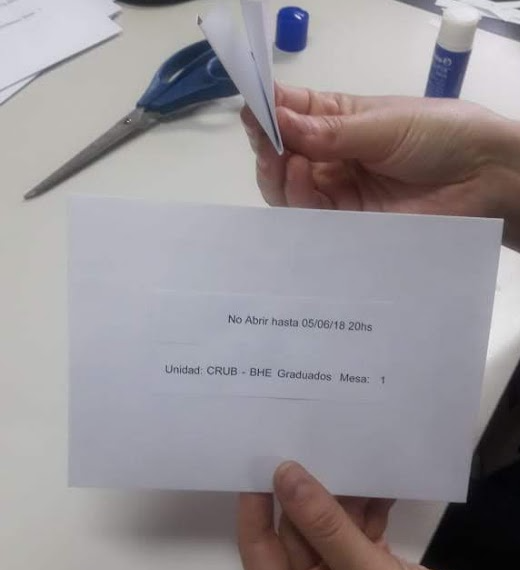
\includegraphics[scale=0.5]{img/jKz6EB2F9Z.png}
    \end{center}
  \caption{Ejemplo Sobre enviado dentro de la urna de la mesa nº1}
  \label{graf:ejemploSobre}
\end{figure}

\item Paso 4: Envío de material. Se envía a cada dependencia el material necesario para poder llevar a cabo los comicios, incluyendo un breve instructivo de carga para la Autoridad de Mesa y el sobre cerrado nombrado en el paso anterior (que sólo debe ser abierto al momento de cargar el acta en el sistema).
\item Paso 5: El Acto Electoral se lleva a cabo en las fechas fijadas por el cronograma electoral y cumpliendo con lo especificado en la Ordenanza Nº 1386/13.
\item Paso 6: Escrutinio Provisorio de la Mesa. 
Una vez que haya finalizado el Acto Electoral, las Autoridades de Mesa realizan el escrutinio provisorio de los votos obtenidos en su mesa, para luego completar por duplicado el acta en papel con la información obtenida del recuento. Ejemplo de un acta cargada en la Figura \ref{graf:ejemploActa}.

\begin{figure}[h!]
    \begin{center}
        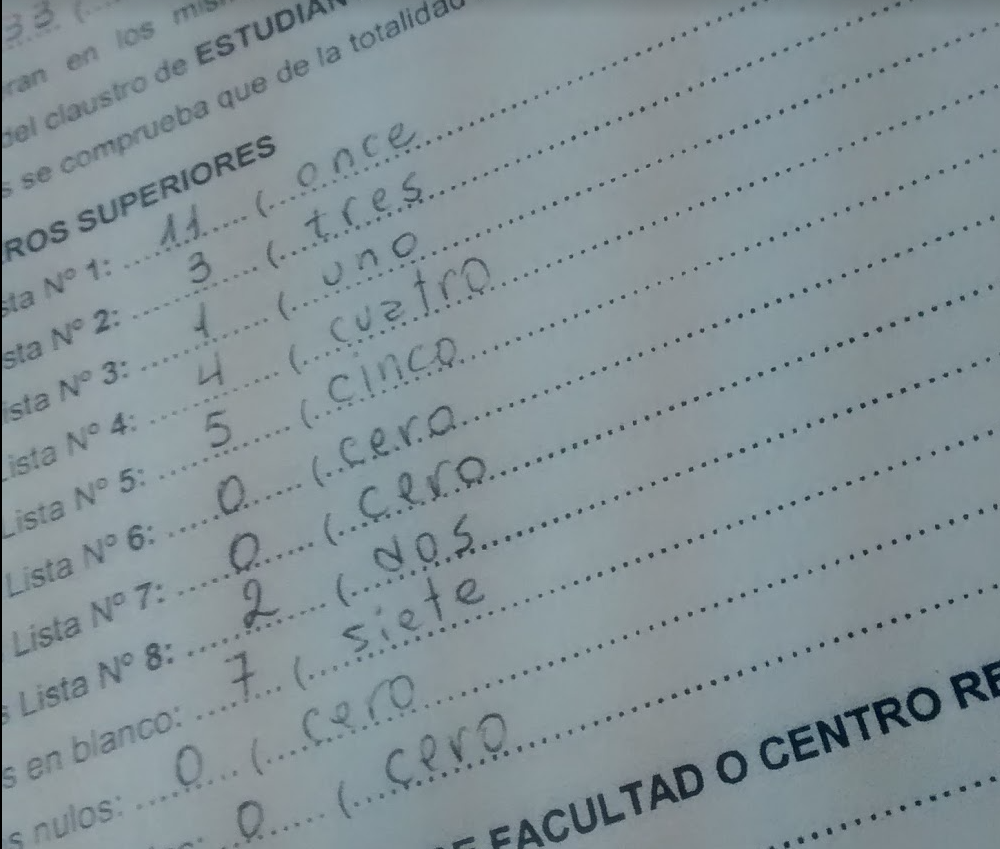
\includegraphics[scale=0.25]{img/f4P4qmrKXY.png}
    \end{center}
  \caption{Ejemplo Acta en papel completada por una Autoridad de Mesa}
  \label{graf:ejemploActa}
\end{figure}

\item Paso 7: Finalizado el Acto Electoral, se habilita el Sistema Gukena para que pueda ingresar cada Autoridad de mesa.
\item Paso 8: Carga y envío de datos en Gukena. Una vez que haya completado el acta papel, la Autoridad de Mesa carga la información de ésta en el Sistema Gukena. Para esto deben ingresar al mismo utilizando el usuario y contraseña contenidos en el sobre. Ejemplo de la pantalla del login en la Figura \ref{graf:ejemploLogin}.
Cuando los datos del acta son confirmados o enviados por la Autoridad de Mesa, estos datos ya no pueden ser editados por este usuario.

\begin{figure}[h!]
    \begin{center}
        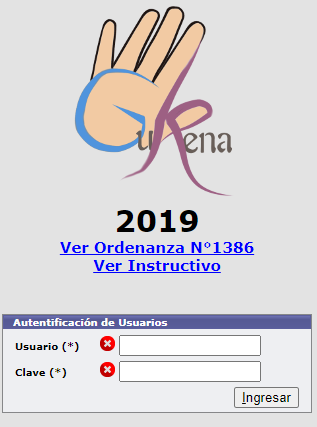
\includegraphics[scale=0.5]{img/ZJ3mtjmmdZ.png}
    \end{center}
  \caption{Pantalla de login para el módulo Autoridad de Mesa y Junta Electoral}
  \label{graf:ejemploLogin}
\end{figure}

\item Paso 10: La Autoridad de Mesa deposita un ejemplar del acta dentro de la urna antes de cerrarla y otro ejemplar es enviado a la Junta Electoral, enviada por los medios disponibles por la Autoridad de Mesa, por ejemplo fax, email, entre otros. 
\item Paso 11: Primera Validación de datos. La Junta Electoral confirma en el sistema que los datos cargados, por las autoridades de mesa, coinciden con las actas papel recibidas, permitiendo corregir cualquier error ocurrido durante el proceso de carga. Para aquellas actas que, por algún inconveniente, no fueran cargadas por la Autoridad de Mesa, como se especifica en el paso anterior, deben ser cargadas por algún miembro de la Junta Electoral.
\item Paso 12: Segunda Validación de los datos. La Secretaria de la Junta Electoral realiza una segunda validación de las actas ya confirmadas por la Junta, en el caso de encontrar diferencias devuelve el acta a la Junta Electoral para su corrección. Si no hay diferencias, entonces dicha acta queda confirmada en el sistema. Una vez que el acta es confirmada ya no puede ser modificada por ningún miembro de la Junta Electoral.

\end{itemize}

A partir del cierre de las mesas de votación, se habilita al público toda la información enviada a través de Gukena, con los resultados parciales (datos enviados por las Autoridades de Mesa) y finales (datos confirmados por la Secretaria de la Junta Electoral).

\section{Proceso de desarrollo}
Utilizar una metodología adecuada al momento de un desarrollo es importante para lograr el objetivo del producto final. Existen muchas metodologías tradicionales y ágiles, estas últimas permiten un proceso de desarrollo más rápido con la intención de no afectar la calidad del producto. Una metodología ágil consiste en un desarrollo incremental con iteraciones muy cortas, beneficiando principalmente a proyectos con requisitos cambiantes y con exigencias en los tiempos
de desarrollo. Brevemente la metodología ágil SCRUM estructura el desarrollo en ciclos llamados Sprints. Estos ciclos son de 1-4 semanas, son de duración fija sin importar si se terminó con el trabajo o no. Al inicio de un sprint, un equipo decide que elementos involucrar y se comprometen terminar al finalizar el sprint. Los elementos elegidos no se pueden cambiar y todos los días el equipo se reúne para informar el avance \cite{scrum}.

Gukena ha sido construido por el Grupo de Desarrollo Euclides\footnote{http://euclides.uncoma.edu.ar/?q=somos} que está integrado por un conjunto de no docentes, estudiantes avanzados y docentes de la Facultad de Informática de la UNComa y funciona bajo la dirección de la Subsecretaría de Tecnologías de la Información de la misma Universidad.

A continuación se detallan las fases de desarrollo ejecutado para lograr el producto final Gukena, estas fases son Análisis, Diseño, Desarrollo y Testing.

\section{Análisis}

En el desarrollo de Gukena se utilizó la metodología SCRUM y el equipo que participó en cada sprint se describe en detalle más adelante (Sección \ref{DesarrolloGukena}). Gukena atravesó 5 iteraciones, cada iteración duró 4 semanas de desarrollo con reuniones semanales para informar el avance. 
Por cada sprint Gukena fue evolucionando incrementalmente integrando nuevas funcionalidades. A continuación se describe el trabajo realizado en cada sprint:

\subsubsection{Sprint 1 (transitado en el año 2015)}

\begin{enumerate}    
    \item Investigación y aprendizaje sobre el proceso y normativo de elecciones en la UNComa y el uso del método D'Hondt.
    \item Diseño y modelado de la base de datos utilizando una base de datos relacional.
    \item Preparación del ambiente de trabajo, utilizando framework Toba y gestor de base de datos PostgreSQL.
    \item Creación de controladores para el formulario de carga de una Autoridad de Mesa.
    \item Creación de controladores para la grilla de mesas con sus estados.
    \item Creación de controladores para el resultado del escrutinio.
    \item Validación del sistema contra el archivo xls utilizado en el escrutinio oficial.
\end{enumerate}
\subsubsection{Sprint 2 (transitado en el año 2016)}
\begin{enumerate}
    \item Análisis y modelado de los datos involucrados en el control de acceso al sistema.
    \item Investigación e integración de seguridad utilizando la herramienta de login que provee el framework Toba
    \item Unión del modelado de datos referidos al control de acceso con la herramienta de login.
    \item Integración con registros de seguimiento sobre actualizaciones en los datos por parte de cada usuario logueado.
    \item Preparación de datos para las elecciones de este año.
    \item Testeo final sobre la funcionalidad en la carga de datos por Autoridades de mesa y su resultado final.
\end{enumerate}
\subsubsection{Sprint 3 (transitado en el año 2017)}
\begin{enumerate}
    \item Preparación de datos para las elecciones de este año (Carta marina).
    \item Testeo final sobre la funcionalidad en la carga de datos por Autoridades de mesa y su resultado final.
    \item Preparación del documento que especifica el Procedimiento de Gukena dentro del marco de elecciones en la UNComa.
\end{enumerate}
\subsubsection{Sprint 4 (transitado en el año 2018)}
\begin{enumerate}
    \item Nuevo diseño y creación de pantallas accesibles por el público en general.
    \item Adaptación del sistema para crear archivos JSON (JavaScript Object Notation) con datos que serán consumidos por nuevas pantallas de Resultados.
    \item Creación de script encargado de copiar los archivos JSON entre dos servidores, desde el servidor procesador de los datos cargados por Autoridad de mesa y Junta Electoral hacia el servidor público con la visualización de los resultados.
    \item Preparación del ambiente de trabajo, esto involucra ambos servidores junto al script y datos dentro del sistema (Carta marina).
    \item Testeo final sobre la funcionalidad en la carga de datos por Autoridades de mesa y su resultado final.
\end{enumerate}
\subsubsection{Sprint 5 (transitado en el año 2019)}
\begin{enumerate}
    \item Preparación del ambiente de trabajo, esto involucra ambos servidores junto al script y datos dentro del sistema(Carta marina).
    \item Testeo final sobre la funcionalidad en la carga de datos por Autoridades de mesa y su resultado final.
    \item Preparación de un documento que especifica los datos accesibles públicamente en los archivos JSON.
\end{enumerate}

\subsection{Historias de usuario en Gukena}

Las Historias de Usuario son un enfoque de requerimientos ágil, estas describen brevemente las características que el sistema debe poseer, requisitos funcionales o no funcionales, narradas desde la perspectiva de la persona que desea dicha funcionalidad.
 Cada historia de usuario establecida en Gukena es comprensible y delimitada para que el desarrollo pueda llevarse a cabo en unas semanas. A continuación se listan las historias de usuario que formaron parte de Gukena:
% \propuesta{REVISAR: se modificaron las historias de usuario}
 \begin{enumerate}
     \item Como Secretaria de la Junta electoral quiero organizar los votos para mejorar la carga.
     \item Como Junta Electoral quiero organizar el escrutinio para validar los datos de manera eficiente.
     \item Como Autoridad de mesa quiero enviar la información del acta para que mejorar el tiempo del proceso.
     \item Como Público quiero ver los resultados de las elecciones para conocer de manera rápida y transparente la información.
     \item Como Equipo de desarrollo quiero ver los registros de operaciones dentro del sistema para disponer fácilmente de ellos por posibles fallas o estadísticas.
 \end{enumerate}
 \begin{comment}
 \begin{enumerate}
     \item Armado de Carta Marina: Esto es la precarga de datos de las listas oficializadas, la distribución de centros de votación (las mesas) junto con la cantidad de electores en cada uno de ellas.
     %\agregar{cv agregar aunque sea una nota al pie diciendo lo que es una Carta Marina} 
     \item ABM Acta de Junta Electoral
     \item Vista de resultados con login
     \item ABM Acta de Autoridad de Mesa
     \item Validación de actas de Junta Electoral
     \item Login de todos los usuarios y auditoría de sus acciones
     \item Resultados públicos
 \end{enumerate}
 \end{comment}
 
\section{Diseño}
%\cambiar{Sección 4.2 se presenta la arquitectura de Gukena pero no se explica en profundidad. La fig. 4.1 representa una arquitectura? A su vez deben estar introducidas las secciones que están contenidas en la misma. Mezcla arquitectura, modelos de datos, con atributos de calidad como seguridad e interoperabilidad. - HECHO: se cambia la palabra arquitectura}
El diseño de un software se compone de un conjunto de principios, conceptos y prácticas para lograr un producto con mejor calidad. El diseño permite representar el sistema que se quiere desarrollar previo a generar lineas de código, una de estas representaciones son los componentes del sistema. A continuación se describe esta representación. 

%\agregar{un párrafo que describe el concepto de diseño y una breve descripción de la Sección.}
\subsection{Estructura del Sistema}
%\propuesta{Le cambié el titulo a Estructura del Sistema, antes era Arquitectura, les parece bien?}
\begin{figure}[h!]
  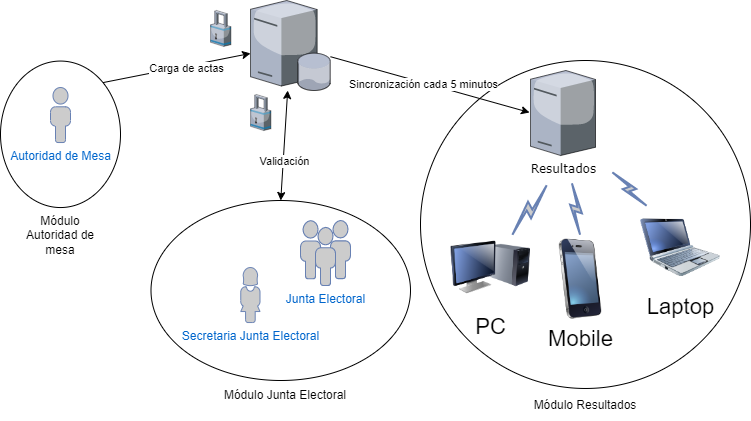
\includegraphics[width=\textwidth]{img/arquitecturaGukena.png}
  \caption{Diagrama de Módulos Gukena}
  \label{graf:arquitectura}
\end{figure}

Gukena se implementó sobre un sistema dividido en tres módulos (Figura \ref{graf:arquitectura}), cada uno se relaciona con los diferentes roles que interaccionan con el sistema.
\begin{itemize}
\item Módulo Autoridad de Mesa: desde cualquier dispositivo con conexión a Internet las Autoridades de Mesa acceden con su usuario y clave para cargar los datos del acta desde el lugar de votación.
\item Módulo Junta Electoral: los integrantes de la junta electoral y la Secretaria realizan un doble chequeo de las actas cargadas por las Autoridades de Mesa en una red interna.
\item Módulo Resultados: muestra los resultados en un servidor web público, para que la comunidad universitaria pueda conocer los resultados a medida que se van cargando los datos.
\end{itemize}

Gukena distingue dos roles para Junta Electoral y Secretaria de la Junta Electoral, sin embargo, se agrupan dentro del mismo módulo. Además, por seguridad la verificación de la Junta Electoral y la confirmación de la Secretaría se realizan dentro de una misma red interna.

Por otro lado, no existe un enlace directo entre los datos del escrutinio cargado al sistema y los datos visualizados por el público. Los datos procesados son depositados en archivos con formato JSON en un servidor de acceso público, los cuales son actualizados continuamente cada 5 minutos por un script interno, estos archivos son consumidos por la página web de resultados para su visualización al público.

La propiedad de usabilidad es importante para que un sistema sea fácil de aprender y de utilizar. Cada uno de estos módulos implican actividades disjuntas dentro del sistema, por lo tanto, para cada rol se le dispuso una interacción distinta con el sistema. \newline
El público en general tiene la necesidad de ver los resultados parciales durante el proceso de escrutinio, para cumplir este objetivo se accede a Gukena a través del sitio público de resultados\footnote{\url{https://resultados.uncoma.edu.ar}}, como se puede ver en la Figura \ref{graf:gukena2019}.
Esta página es accesible desde cualquier navegador, contiene categorías de búsqueda de información (1), gráficos (2), descripciones explicativas sobre los datos visualizados (3), avance de carga de mesas por las autoridades de mesa o validadas por la Junta Electoral (4) y fecha/hora de los datos procesados que se están visualizando (5). 

\begin{figure}[h!]
  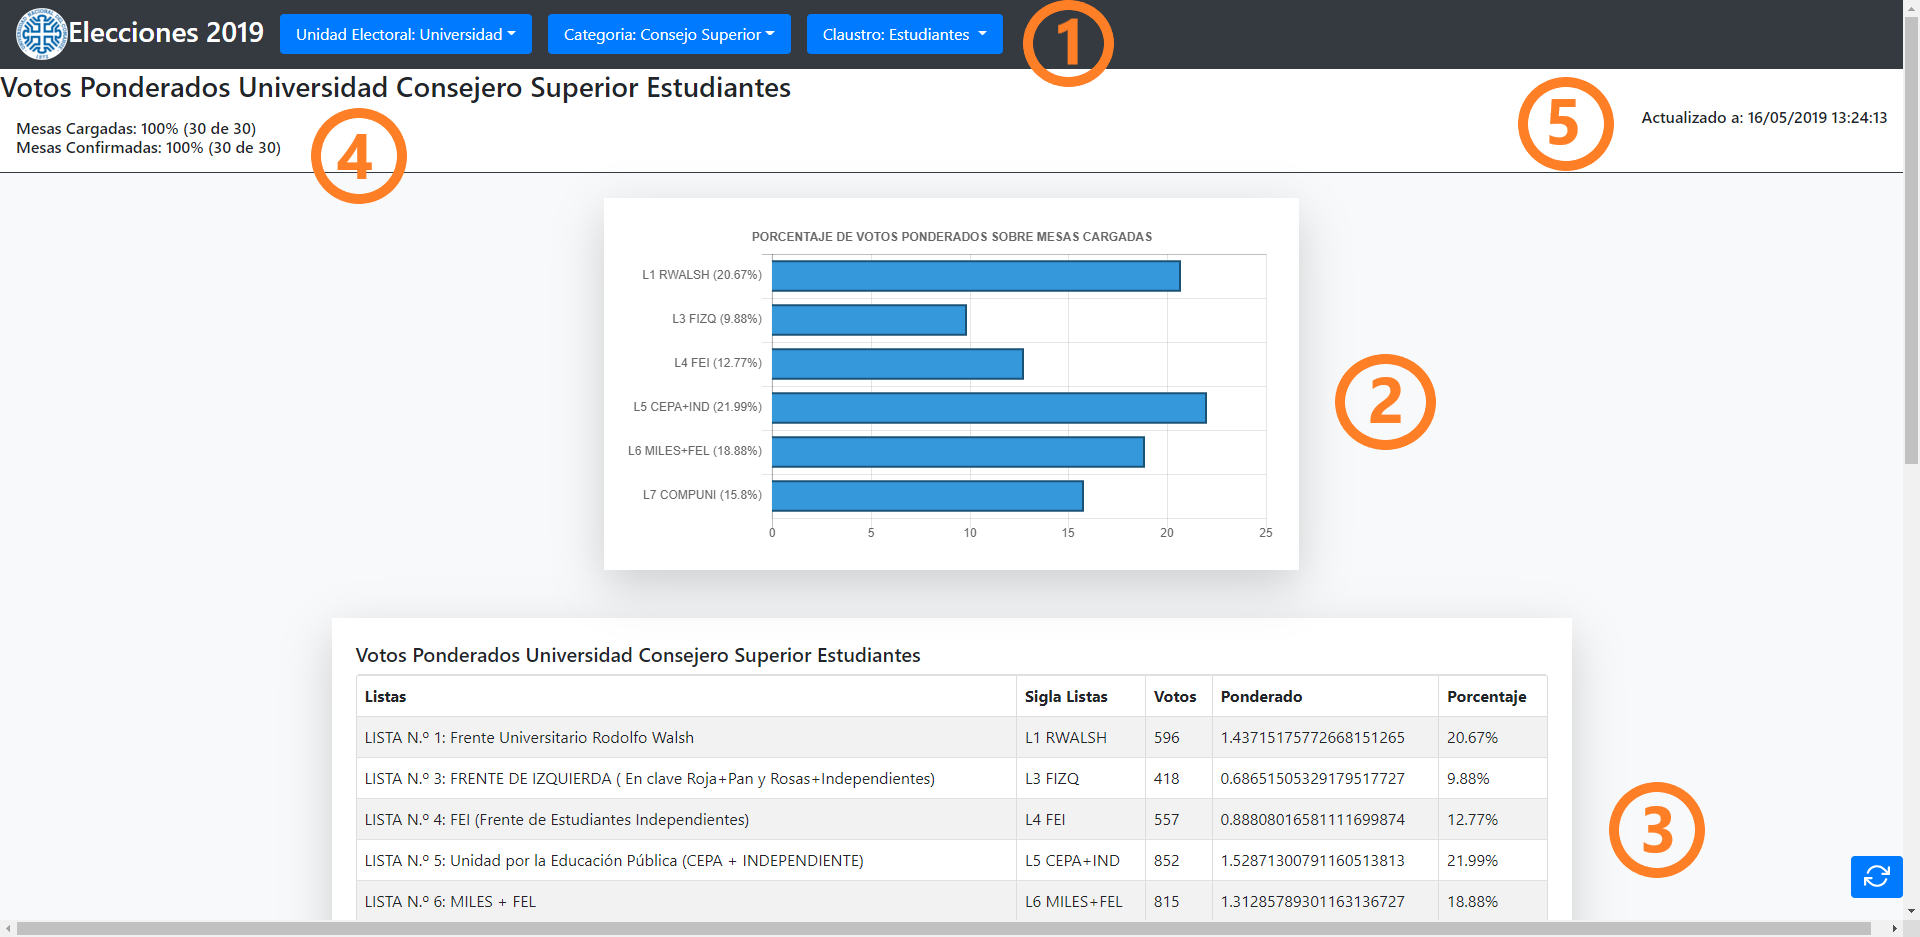
\includegraphics[width=\textwidth]{img/resultados_tags.png}
  \caption{Resultados elecciones UNComa en el año 2019}
  \label{graf:gukena2019}
\end{figure}

Por otro lado, el rol de autoridad de mesa tiene la necesidad de transmitir la información del resultado de su escritinio, por este motivo acceden al formulario de carga\footnote{\url{https://gukena.fi.uncoma.edu.ar/}}, como ejemplo en la Figura \ref{graf:formularioGukena}, se loguean con la información recibida previamente y acceden a una única pantalla con un formulario correspondiente a la mesa escrutada. 
Como se puede ver en la Figura de ejemplo, la autoridad de mesa puede visualizar el claustro, unidad electoral, sede, número de mesa y cantidad de empadronados de la mesa correspondiente. Luego se disponibiliza el formulario de carga por cada lista oficializada y las acciones de Guardar/Enviar para transmitir los datos cargados.

Por último, tenemos al módulo de Junta Electoral quienes necesitan validar y/o corregir la información cargada en el sistema. Acceden al mismo link que una autoridad de mesa con la diferencia que al validar múltiples mesas, el sistema le dispone un listado de todas las mesas, con filtros y categorías para facilitar su búsqueda. 
Como se puede ver en la Figura \ref{graf:grillaGukena}, cada mesa se encuentra etiquetada con información sobre su estado, es decir, si ya fue cargada por la autoridad de mesa correspondiente, en la espera de su carga o si ya fue validado. Por cada mesa se le despliega la misma pantalla que se dispone a una autoridad de mesa para que pueda hacer las correcciones necesarias con una acción de validar esta información. \newline

\begin{figure}[h!]
    \begin{center}
        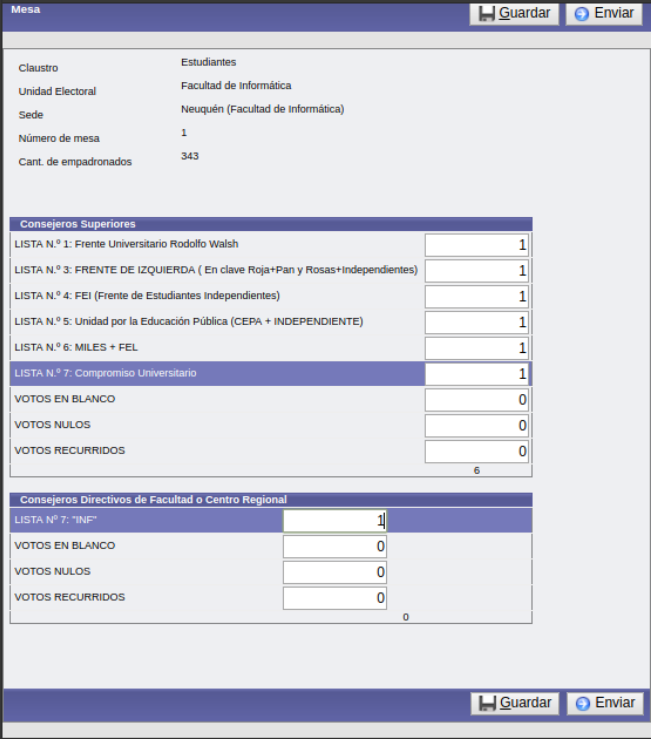
\includegraphics[width=0.9\textwidth]{img/jvFvvu4LpJ.png}
    \end{center}
  \caption{Ejemplo formulario de carga}
  \label{graf:formularioGukena}
\end{figure}

\begin{figure}[h!]
    \begin{center}
       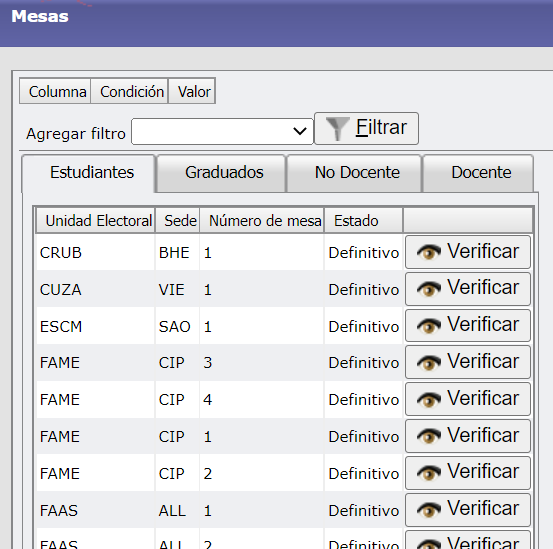
\includegraphics[width=0.6\textwidth]{img/ejemploGrillaMesasGukena.png}
    \end{center}
  \caption{Ejemplo grilla de mesas para validar}
  \label{graf:grillaGukena}
\end{figure}


Cabe destacar que una autoridad de mesa solo tiene disponible el formulario de carga hasta que envía la información cargada, a partir de ese momento solo puede visualizar el formulario pero no volver a editarlo.\newline 
Por otro lado, a nivel técnico Gukena se desarrolló sobre una infraestructura web LAPP (Linux Apache PostgreSQL PHP):
\begin{itemize}
    \item Linux\footnote{https://www.linux.org/}: Sistema Operativo basado en software libre.
    \item Apache\footnote{https://www.apache.org/}: Servidor web.
    \item PostgreSQL\footnote{https://www.postgresql.org/}: Servidor de base de datos relacionales open source.
    \item PHP\footnote{https://www.php.net/}: Lenguaje de programación open source embebido en páginas HTML, ejecutado en el servidor. Compatible con distintos sistemas operativos y bases de datos.
\end{itemize}
Se eligieron estos componentes de LAPP ya que son de código abierto completo, es segura y estable. Además existe una amplia comunidad que ofrece un gran soporte ante cualquier inconveniente. 

Durante el desarrollo se utilizan solamente herramientas de software libre, por este motivo, se usa el ambiente de desarrollo web SIU Toba \footnote{https://www.siu.edu.ar/siu-toba/}, desarrollado por el consorcio SIU para soluciones del Sistema Universitario Nacional. Esta herramienta
permite crear sistemas transaccionales en forma rápida, utilizando tecnología web open-source y su objetivo es agilizar el proceso de construcción y el mantenimiento de los mismos. De esta manera, permite al equipo de desarrollo enfocar su actividad en la lógica del dominio. El ambiente de desarrollo web SIU Toba está basado en el patrón arquitectónico MVC el cual separa los datos de una aplicación, la interfaz de usuario y la lógica de control en tres componentes distintos: Modelo, Vista, Controlador. Estos componentes se explican más adelante con mayor detalle. Una de las ventajas de esta arquitectura MVC es permitir separar los componentes de una aplicación dependiendo de la responsabilidad que tienen, respetando el principio de la responsabilidad única.


\subsection{Modelo de datos}

La semántica de este problema se representó sobre una base de datos relacional utilizando herramientas de software libre. Se utilizó el Gestor de Base de Datos PostgreSQL sobre un sistema operativo Linux. El modelo de datos representa los conceptos más importantes en un dominio. En el proceso de elección en la UNComa se observan las entidades más importantes que son: unidad electoral, mesas, claustros, actas y las listas oficializadas para cada cargo.
El modelo de datos representado en la Figura \ref{graf:diagramaBD} es el almacenamiento principal del sistema, es decir, la carga de datos por parte de las autoridades de mesa y Junta Electoral y, el procesamiento de los resultados impacta sobre esta fuente de datos. La documentación de la base de datos se encuentra disponible con más detalle en el Anexo \ref{DBGukena}.

En base a estos conceptos principales tenemos los votos que recibe cada lista postulada agrupadas por las sedes que conforman cada Unidad Electoral. Además para mantener el histórico de elecciones se tiene la entidad Acto Electoral manteniendo las fechas de cada elección realizada.\newline
Conociendo el modelo de datos, al momento de una nueva elección es necesario realizar una precarga de datos sobre:
\begin{itemize}
    \item Acto electoral con fecha de la nueva elección, asociando los claustros que votarán y las unidades electorales y sedes participantes.
    \item Datos de las mesas: número de mesa, cantidad de empadronados en cada mesa, claustro al que pertenece.
    \item Listas oficializadas para cada claustro y el cargo al que se postula.
    \item Usuarios habilitados a ingresar al sistema.
\end{itemize}
La entidad Mesa tiene 5 estados:
\begin{itemize}
    \item No Cargado.
    \item Cargado.
    \item Enviado.
    \item Confirmado.
    \item Definitivo.
\end{itemize}

Al momento de la precarga de datos, la mesa se encuentra en estado inicial ``No Cargado'' (id\_estado = -1). Cuando la Autoridad de Mesa carga la información de su acta y lo guarda, la mesa transiciona al estado ``Cargado'' (id\_estado=1). Al momento que la Autoridad de Mesa envía esta información, el estado de la mesa pasa a ``Enviado'' (id\_estado=2), en este estado no se podrán modificar los datos de la mesa por la Autoridad de Mesa. La Junta Electoral valida la información de la mesa y pasa al estado ``Confirmado'' (id\_estado=3), ésta es la primera validación que reciben los datos. La Secretaria de la Junta Electoral confirma esta información y la mesa pasa al estado ``Definitivo'' (id\_estado=4), segunda validación de los datos, en este estado no se podrán modificar los datos por ningún rol, la información ya forma parte de los resultados definitivos.

%\cambiar{La Figura 4.4 es ilegible y no está explicada. - HECHO: se actualiza la imagen, veo que estaba actualizada, que más agregar??}
\begin{figure}[h!]
  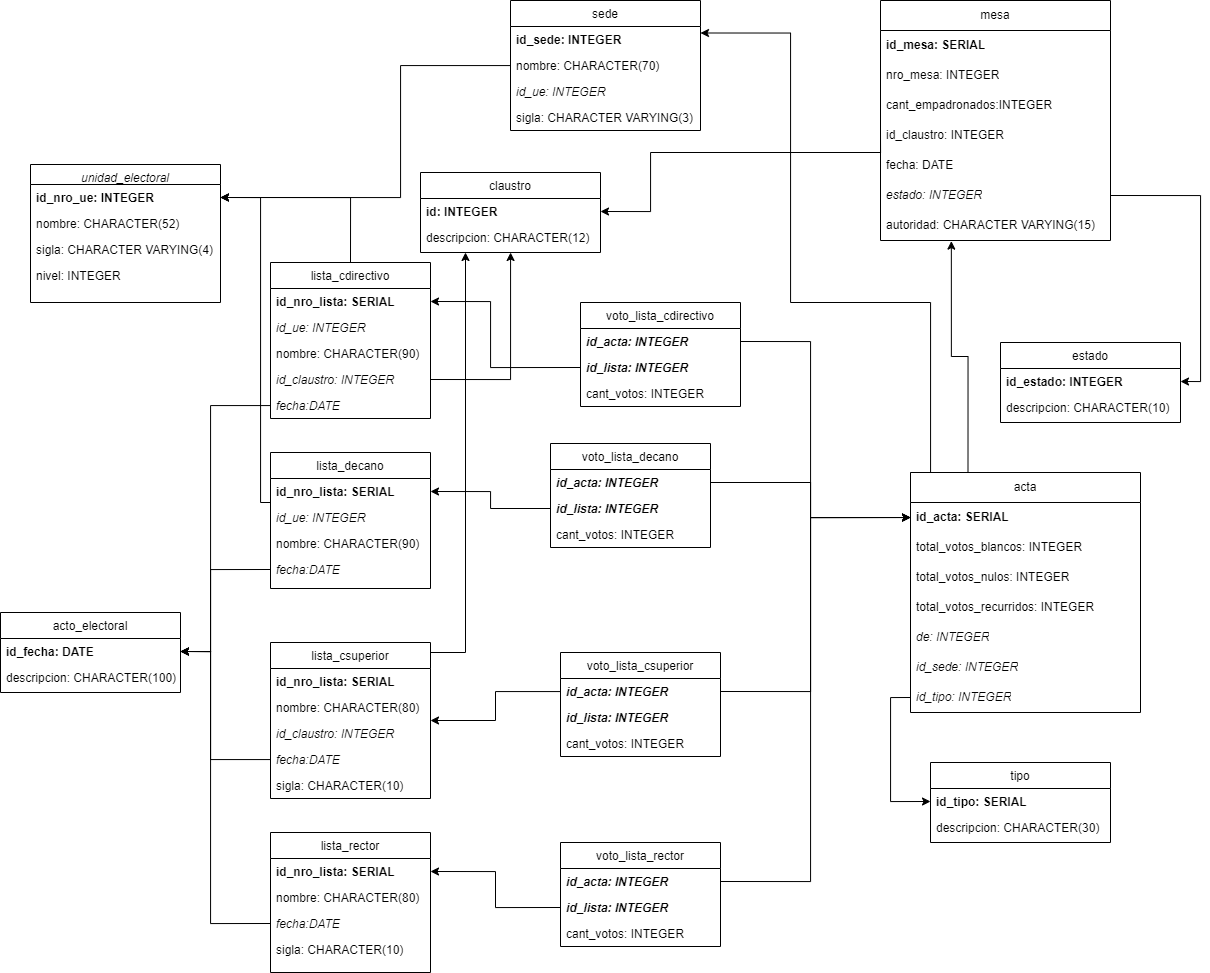
\includegraphics[width=\textwidth]{img/merGukena.png}
  \caption{Relación entre las tablas almacenadas en la Base de Datos Gukena}
  \label{graf:diagramaBD}
\end{figure}

\subsection{Interoperabilidad externa}

Un programa ejecutado del lado cliente se comunica con los servicios web a través de APIs (Application Programming Interfaces). Las APIs exponen un conjunto de datos y funciones para facilitar la interacción entre programas y así poder intercambiar información, además de dar una capa de seguridad sobre los datos reales almacenados. El estilo de arquitectura REST es aplicado comúnmente en el diseño de APIs de servicios web modernos. Por lo tanto, una API web implementado con esta arquitectura es un API REST \cite{masse2011rest}.

Gukena expone este conjunto de datos a través de archivos en formato JSON con una arquitectura propia que permite su fácil consulta desde programas cliente. Estos archivos son actualizados durante el escrutinio cada 5 minutos y son el resultado de procesar los datos existentes en la base de datos SQL. Estos archivos son consumidos por la página pública de resultados de Gukena, sin embargo, pueden ser consultados por cualquier sistema o persona que los quiera acceder. 
Como se muestra en la tabla \ref{tab:formatoJSON}, para reconocer qué archivo se debe consumir para obtener los datos deseados,  se aplicó la siguiente notación en el nombre de cada archivo:  

\emph{Cargo + `\_' + Unidad Electoral + `\_' + Claustro + ``.json''} \newline
A continuación se describe brevemente la estructura interna de estos archivos:
\begin{itemize}
    \item data 
    \begin{itemize}
        \item lista (String)
        \item sigla (String)
        \item total de votos (int)
        \item sede (int)
    \end{itemize}
    \item columns 
    \begin{itemize}
        \item field (String)
        \item title (String)
    \end{itemize}
    \item titulo (String)
    \item labels (String)
    \item total (int)
    \item fecha (datetime)
    \item enviados y confirmadas (String)
    \item titulo\_grafico (String)
\end{itemize}




\begin{table}[htbp]
\begin{center}
\begin{tabular}{|l|l|l|}
\hline
Cargo & Unidad Electoral &  Claustro\\
\hline \hline 
R(Rector) & Todo(Universidad) & T(Total)\\ \hline
D(Decano) & ASMA & D(Docentes)\\ \hline
CD(Consejo Directivo) & AUZA & E(Estudiantes)\\ \hline
CS(Consejo Superior) & CRUB & G(Graduados)\\ \hline
& CUZA & N(No Docentes) \\ \hline
& ESCM & \\ \hline
& FACA & \\ \hline
& FACE & \\ \hline
& FADE & \\ \hline
& FACA & \\ \hline
& FAEA & \\ \hline
& FAHU & \\ \hline
& FAIF & \\ \hline
& FAIN & \\ \hline
& FALE & \\ \hline
& FAME & \\ \hline
& FATA & \\ \hline
& FATU & \\ \hline
\end{tabular}
\end{center}
\caption{Nombre de archivos JSON}
\label{tab:formatoJSON}
\end{table}

\subsection{Seguridad}
Las vulnerabilidades de un software afectan a la seguridad de un sistema, estos pueden ser debilidades funcionales o lógicos.
Descubrir estas vulnerabilidades es importante para proteger la información \cite{definicionVulnerabilidad}.

Se ha contemplado y evaluado la Seguridad en cada fase  del diseño e implementación del sistema.  La principal amenaza es que se vulnere el enlace con los usuarios que cargan y verifican los datos.  Por esta razón, los tres módulos están publicados en un servidor web Apache a través del protocolo HTTPS para asegurar el enlace. Además, la verificación de la Junta Electoral y la confirmación de la Secretaría se realizan dentro de una red interna privada. 

Así mismo, no existe un enlace directo entre los datos del escrutinio cargado al sistema y los datos visualizados por el
público. Los datos procesados son depositados en archivos con formato JSON los cuales son actualizados continuamente cada 5 minutos por un script interno, estos archivos son consumidos por la página web de resultados para su visualización al público. 

Existe una fundación sin fines de lucro OWASP\footnote{https://owasp.org/} (Open Web Application Security Project) cuyo objetivo es mejorar la seguridad del software. OWASP Top 10 es un documento estándar de conscientización para desarrolladores sobre la seguridad en aplicaciones web. El documento contiene los 10 riesgos más críticos en seguridad, el ranking obtenido en el 2020 se representa en la tabla \ref{tab:top10}.

\begin{table}
\begin{center}
\resizebox{\textwidth}{!}{
  \begin{tabular}{p{0.35\textwidth}p{0.65\textwidth}}
    \toprule
Riesgo & Prevención\\
    \midrule
    1.Inyección & \tabitem Parametrizar las consultas \\
    & \tabitem Validar los datos ingresados  \\
    & \tabitem Escapar caracteres especiales  \\
    \hline
    2.Autenticación rota & \tabitem Usar buenas librerias de autenticación\\
    & \tabitem Forzar el uso de contraseñas fuertes \\
    & \tabitem Detectar y prevenir ataques de fuerza bruta \\
    \hline
    3.Datos sensibles expuestos & \tabitem No guardar datos que no se necesiten\\
    & \tabitem Usar un encriptado fuerte \\
    \hline
    4.XML Entidades Externas (XXE) & \tabitem Evitar XML\\
    & \tabitem Usar librerías modernas con una buena configuración \\
    & \tabitem Validar XML \\
    \hline
    5.Control de acceso rota & \tabitem Usar códigos o librerías probadas\\
    & \tabitem Por defecto denegar el acceso \\
    & \tabitem Guardar fallas y alertar \\
    & \tabitem Acceso limitado en accesos a recursos \\
    \hline
    6.Mala configuración de seguridad & \tabitem Deshabilitar servicios no usados\\
    & \tabitem Usar herramientas para revisar configuraciones \\
    \hline
    7.Cross-site Scripting (XSS) & \tabitem Codificar todos los datos recibidos del usuario\\
    & \tabitem Usar una codificación apropiada al contexto \\
    & \tabitem Usar frameworks que genere HTML seguro \\
    & \tabitem Usar política de seguridad de contenido \\
    \hline
    8.Deserealización insegura & \tabitem Evitar serializar y deserealizar objetos\\
    & \tabitem Usar firmas para detectar manipulaciones\\
    & \tabitem Configurar librerias seguras \\
    & \tabitem Limites de accesos a recursos \\
    \hline
    9.Utilización de componentes con vulnerabilidades conocidas 
    & \tabitem Reducir dependencias\\
    & \tabitem Parches admnistradas \\
    & \tabitem Escanear componentes vencidos\\
    & \tabitem Presupuestar por el mant. continuo de todos los proyectos de software \\
    \hline
    10.Logging y monitoreo insuficientes \\
    \bottomrule
  \end{tabular}
  }
  \end{center}
  \caption{OWASP Top 10}
\label{tab:top10}
\end{table}


Como se puede ver existen distintos tipos de ataques a los datos de un sistema con el fin de obtener información, manipularlos o destruirlos. El término Inyección por SQL consiste en la inserción de código SQL por medio de los datos de entrada desde el lado de cliente hacia el servidor. Es decir, por medio de la inserción de este código el atacante puede modificar las consultas originales que debe realizar la aplicación y ejecutar otras totalmente distintas con la intención de acceder a la herramienta, obtener información de alguna de las tablas o borrar los datos almacenados, entre otras acciones malintencionadas. Al conocer este término se puede ver que debido a que la página utiliza archivos para alimentarse y no realiza consultas SQL directas a la base de datos, este tipo de ataque no es posible. Como mayor daño podría llegar a ser manipular o destruir estos archivos, que luego son reemplazados nuevamente de manera automática por el sistema con los datos reales y correctos. 

Otro de los ataques que se nombran es el acceso no autorizado al sistema con el objetivo de manipular los datos cargados del escrutinio en una mesa en particular, o un conjunto de ellas. Los usuarios con los roles de Autoridad de mesa, Junta Electoral y Secretaría inician sesión con nombre de usuario y clave para ingresar al sistema. Esta información confidencial fue recibida de manera impresa dentro de un sobre cerrado con la instrucción de que la persona encargada del cierre de la mesa de votación debe abrirlo para ingresar al sistema. Además se registra cada acción de inserción y modificación que se realiza en los formularios del sistema en un registro (log) general para cubrir el riesgo 10 nombrado en el ranking. \newline

\section{Desarrollo}
\label{DesarrolloGukena}

Gukena ha sido construido por el Grupo de Desarrollo Euclides. El sistema se desarrolló durante los meses de abril a junio a partir del 2015 y los años siguientes, integrándose mejoras evolutivas en cada año.

Quien planteó la necesidad sobre el proceso electoral en la UNComa fue la Secretaria del Consejo Superior María Elena Sandoval. La experta del dominio ha sido de ayuda para formalizar este sistema, quien además es la principal beneficiada, porque antes de la existencia de Gukena, la administración de los resultados de las elecciones dependían de una única planilla de cálculo gestionada por la secretaria. Otro integrante principal ha sido el docente Claudio Vaucheret quien impulsó el sistema descentralizado con respecto a la carga de las actas en cada mesa de votación.

El proyecto ha sido dirigido por el docente Pablo Kogan y no docente Andrea Granados. \newline
A continuación se nombran las personas que aportaron a la evolución del desarrollo de Gukena por cada año, tanto a nivel de desarrollo como análisis y diseño. Además se detalla mi participación en cada año.
\subsubsection{2015}
Equipo integrado por:
\begin{itemize}
    \item Bruno Guala
    \item Valeria Zoratto
    \item Silvia Soto
\end{itemize}

Este año fue un acercamiento al objetivo, sin embargo, solo se llegó a un prototipo de Gukena sin llegar a ser implementado en la UNComa. Durante este periodo tuve participación activa en la investigación, aprendizaje del proceso normativo y uso del método D'Hondt. Además participé en el diseño y modelado de la base de datos, aprendizaje del framework SIU Toba y preparación del ambiente. También participé en la creación de los componentes necesarios para el formulario de carga (correspondiente a las Autoridades de Mesa), la grilla de las mesas para validar (correspondiente al rol de Junta Electoral y Secretaria) y la pantalla de resultados.

\subsubsection{2016}
Equipo integrado por:
\begin{itemize}
    \item Bruno Guala
    \item Celeste Ramos
    \item David Troncoso Schenker
    \item Silvia Soto
\end{itemize}

Este año fue el primer año cuando Gukena se integró al proceso electoral de la UNComa. Durante este periodo de desarrollo, participé en la investigación y utilización de la herramienta de login integrado en SIU Toba. Además participé en la preparación de los datos para las elecciones, testeo final sobre el funcionamiento general del sistema y procesamiento de los resultados. Durante el periodo de escrutinio, participé junto a la Secretaria de la Junta Electoral, como soporte durante las validaciones finales de las actas con los datos cargados en el sistema.

\subsubsection{2017}
Equipo integrado por:
\begin{itemize}
    \item Celeste Ramos
\end{itemize}

Durante este año no hubo grandes cambios en Gukena, sin embargo, tuvo lugar la preparación del Procedimiento de Gukena dentro del proceso electoral de la UNComa, además de la preparación de los datos para las elecciones. Durante este período participé durante el periodo de escrutinio como soporte para visualizar los resultados de las elecciones de forma presencial.

\subsubsection{2018}
Equipo integrado por:
\begin{itemize}
    \item Bruno Guala
    \item Celeste Ramos
    \item David Troncoso Schenker
    \item César Gutiérrez 
    \item Walter Esparza 
    \item Silvia Soto
\end{itemize}

En este año Gukena tuvo una evolución importante en el diseño y creación de pantallas que están disponibles al público en general. Este año Gukena posee una pantalla de resultados con gráficos, historial y buscadores de las elecciones a partir del año 2015 en UNComa. En esta evolución, tuve participación activa en el desarrollo del Back-End, esto es, obtener, consolidar y enviar los datos procesados a un conjunto de archivos JSON. Estos archivos quedan disponibles para que la pantalla de resultados, desarrollada por el resto del equipo pueda consumirla. Además participé durante el testing final del funcionamiento del sistema, y durante el escrutinio como soporte en las validaciones de la Junta Electoral.

\subsubsection{2019}
Equipo integrado por:
\begin{itemize}
    \item German Kiessling
\end{itemize}

Durante este año no hubo grandes cambios en Gukena, sin embargo, tuvo lugar la preparación del documento especificando la información disponible públicamente en los archivos JSON, además de la preparación de los datos para las elecciones. Durante este período participé durante el periodo de escrutinio como soporte en la comunicación por correo electrónico por parte de las Autoridades de Mesa.

\begin{comment}
\subsubsection{2022}
Equipo integrado por:
\begin{itemize}
    \item Juan Marcos Gonzalez
    \item Santiago Scantamburlo
    \item Lucas Villaruel
\end{itemize}
\end{comment}
%\agregar{Si vos lo consideras 2022 Juan Marcos Gonzalez, Santiago Scantamburlo y Lucas Villaruel}
Además del equipo de desarrollo, Gukena no podría ejecutarse sin la presencia de las personas que formaron parte del equipo administrando los servidores durante todos estos años. En las elecciones los no docentes Luis Coralle y Lic. Alejandro Mora permitieron el acceso y buen funcionamiento de Gukena durante el acto electoral.

En el año 2015 una primera versión prototipo se utilizó para validar las planillas de cálculos usadas hasta el momento por las autoridades de las elecciones, sólo fue utilizado por el equipo de desarrollo en ese momento, no llegando a ser utilizado en la UNComa. En el año 2016 y 2017 se integró Gukena en su totalidad en las etapas de procesamiento, carga de datos en la universidad y publicación de resultados.  En 2018 fue la primera vez que se utilizó en una elección completa considerando los cuatro claustros: Estudiantes, No Docentes, Docentes y Graduados junto con la elección de los cargos de Rector, Decano, Consejeros Directivos y Superiores. Este año se aplicaron mejoras sobre las pantallas accesibles por el público en general que permiten ver los resultados parciales en tiempo real (Figura \ref{graf:gukena2019}), junto a un histórico de elecciones. Esta mejora fue bien aceptada por la comunidad universitaria permitiendo a los medios de comunicación y público en general tener un acceso rápido a los resultados.

En la construcción, diseño e implementación de Gukena se utilizaron solamente herramientas de software libre. En el desarrollo se usa el ambiente de desarrollo web SIU Toba.
Se trabaja utilizando la filosofía del desarrollo de código abierto, para contribuir a mejorar el mantenimiento del sistema. Los fuentes son de licencia libre y acceso público, se encuentran disponibles en el repositorio libre\footnote{\url{https://github.com/svs07uni/gu_kena}} 
con la intención  de que la comunidad de desarrolladores, investigadores, y comunidad de la Universidad puedan acceder al software y analizarlo.

%\cambiar{La figura 4.8 y 4.9 no son necesarias si no están bien explicadas - HECHO: se quita 4.8, se explica 4.9}
\begin{comment}
 
\begin{figure}[h!]
    \begin{center}
        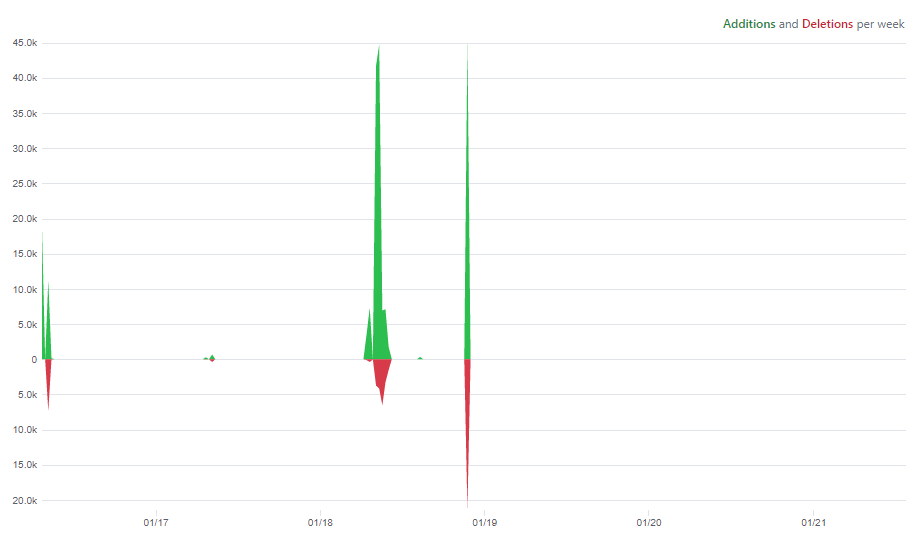
\includegraphics[width=\textwidth]{img/graficoGithub.png}
    \end{center}
  \caption{Github - Code Frecuency}
  \label{graf:codeFrecuency}
\end{figure}
   
\end{comment}

%\agregar{reformular descripción MVC toba con fragmentos de código y gráfico}
El ambiente de desarrollo web SIU Toba está basado en el patrón arquitectónico MVC el cual separa los datos de una aplicación, la interfaz de usuario y la lógica de control en tres componentes distintos:
\begin{itemize}
    \item Model (Modelo): Es la representación de la información con la cual el sistema opera y gestiona todos los accesos a dicha información. En este contexto, el Modelo permite guardar y consultar los datos del escrutinio final por cada mesa, almacenados en la Base de Datos. Además este componente se encarga de aplicar las fórmulas necesarias para conseguir el resultado provisorio y/o final de la distribución de escaños. Otra información importante que gestiona es el registro de actualizaciones sobre estos datos. Esto permite satisfacer las propiedades de auditabilidad, ya que se registran las actualizaciones por parte de las autoridades de mesa y personal de la Junta Electoral autorizada.
    \item View (Vista): Presenta el Modelo de una manera adecuada para interactuar con ella, es decir, la interfaz de usuario. Se encarga de la representación visual de los datos. Gukena dispone una vista por cada módulo de interacción. De manera tal que una autoridad de mesa sólo accede a un formulario de carga, una persona autorizada de la Junta Electoral accede a un listado de mesas a validar, y por último una vista más gráfica para el módulo de Resultados. Este componente tiene la responsabilidad de satisfacer las propiedades de usabilidad del sistema.
    \item Controller (Controlador): Responde a eventos e invoca peticiones al Modelo, se encarga de controlar las acciones del usuario y de solicitar los datos al Modelo para comunicárselos a la vista. En Gukena, el Controlador suministra los datos mediante dos vias, una de ellas es la comunicación directa entre Vista y Modelo para los módulos de Autoridad de Mesa y Junta Electoral. Sin embargo, para el módulo de Resultados el controlador ``empaqueta'' los datos y los deposita en archivos JSON, los cuales son el origen de datos para la Vista.
\end{itemize}

El proceso de cómo interactúan estos tres componentes se puede observar en la Figura \ref{graf:mvcArquitectura}. El primer paso en este proceso es disparada por el usuario (User) capturada por el Controlador (Controller), luego este componente realiza la petición de los datos necesarios al Modelo (Model). Este último accede a la Base de Datos (Database) realizando las transacciones necesarias para luego retornar los datos obtenidos al Controlador. El Controlador suministra toda la información a la Vista (View) quien es la encargada final de armar la experiencia expuesta al Usuario. Todo este proceso es ejecutada por cada petición invocada por el Usuario.

\begin{figure}[h!]
    \begin{center}
        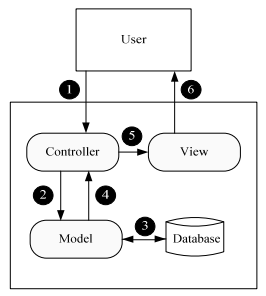
\includegraphics{img/mvc_arq.png}
    \end{center}
  \caption{Arquitectura del Framework SIU Toba}
  \label{graf:mvcArquitectura}
\end{figure}

SIU Toba respeta notaciones para referir a cada uno de estos componentes, por ejemplo en la Figura \ref{graf:ejemploPantalla} se puede ver una parte del código de configuración sobre el controlador asociado a la mesa. Al tener la palabra ``conf'' refiere a la configuración y la palabra ``pant'' se asocia a la pantalla denominada ``edicion''. De igual modo, se puede observar como se accede al Modelo dentro de este framework con la siguiente linea
\begin{lstlisting}
$this->dep('datos')->tabla('nombreTabla')}
\end{lstlisting}
Esta notación ayuda a su mantenimiento ya que el código queda más prolijo y claro.

\begin{figure}[h!]
    \begin{center}
        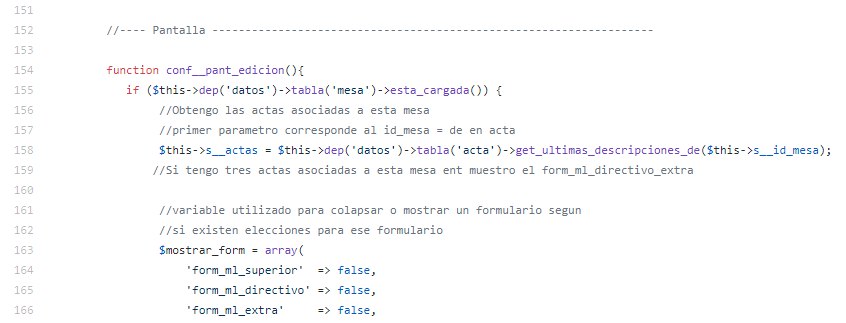
\includegraphics[width=\textwidth]{img/ejemplo_pantalla.png}
    \end{center}
  \caption{CI Mesa - Carga de pantalla de Edición de una mesa}
  \label{graf:ejemploPantalla}
\end{figure}

\section{Testing}
%\cambiar{Sección 4.4 - Testing, podría poner ejemplos del testeo que hicieron y cómo lo llevaron a cabo.}
%\cambiar{El Testing fue trabajo de la tesista o trabajo previos?}
El Testing de un software es cualquier actividad cuyo objetivo es evaluar un atributo o la capacidad de un programa o sistema y determina si logró encontrar los resultados esperados \cite{pan1999software}. Esto no significa que únicamente se utiliza para validar (debuggear) un software, el propósito del Testing es asegurar la calidad, verificación y validación, o estimación de confiabilidad. Esta actividad contiene métodos y técnicas destinadas a múltiples propósitos durante las fases dentro de un desarrollo de software. Testing se puede dividir como: testing de correctitud, testing en performance, testing en confiabilidad y testing de seguridad. Un tester puede abocarse a verificar la correctitud de un sistema o software sin conocer internamente su funcionamiento, conocido como testing de caja negra (black-box testing). O por el contrario, planificar los casos de test de acuerdo a los detalles de implementación del software (testing de caja blanca o white-box testing). 

Para los casos de test en Gukena participó el equipo de desarrollo y usuarios externos a éste, como docentes de la Facultad de Informática. El testing se ejecutó como última etapa previa a la utilización final de Gukena en las elecciones de la UNComa. En esta etapa se crearon usuarios de pruebas utilizados por las personas involucradas en el testing, cada usuario asignado a roles distintos. Parte de los usuarios realizaron testings de correctitud y seguridad, validando el comportamiento en la carga o validación de sus formularios disponibles y el acceso no autorizado. Otra conjunto de usuarios realizaron testings de consistencia en el procesamiento de los datos, esto incluyó la carga de datos en un conjunto reducido de mesas y su verificación en el procesamiento de los resultados parciales y finales obtenidos.

En resumen, los casos de test involucraron:
\begin{itemize}
    \item Carga de datos erróneos en los formularios de carga del rol Autoridad de mesa, por ejemplo valores negativos en los formularios.
    \item Verificar validaciones integradas en los formularios en la pantalla de carga del rol Autoridad de mesa. Por ejemplo las validaciones contra la cantidad de empadronados y/o validaciones en la cantidad de votantes cargadas en cada formulario.
    \item Verificar cambios de estado de una mesa desde el guardado hasta la validación final por el rol Junta electoral.
    \item Verificar los datos procesados por una cantidad reducida de mesas cargadas contra el resultado final generado por el sistema.
    \item Accesos no autorizados por usuarios no permitidos.
    \item Testing de sobrecarga en consultas paralelas con una cantidad reducida de dispositivos en un mismo instante.
\end{itemize}

En esta etapa, participé de forma activa tanto en las pruebas de correctitud en los formularios como en la verificación del procesamiento de los datos.

\section{Conclusión}

Luego de analizar el impacto de la tecnología en las distintas fases del modelo de referencia, podemos decir que Gukena es un sistema que se involucró en las fases menos críticas o si ocurre algún error queda en evidencia y se puede corregir al instante. Estas fases son: 
\begin{itemize}
    \item Escrutinio de la Mesa: sólo como ayuda para verificar datos finales, como por ejemplo la cantidad de votantes no debe superar la cantidad de empadronados en una mesa particular.
    \item Comunicación de Resultados: transmite los datos cargados hacia los servidores internos del sistema.
    \item Procesamiento de Resultados y Publicación.
\end{itemize}

De esta manera Gukena no se involucra en las etapas cercanas al voto individual obligando a que el escrutinio de una mesa sea manual, y que el acta sea en papel firmado por todas las autoridades de la mesa.
 
Algunas características al utilizar Gukena son:
\begin{itemize}
\item Carga distribuida de las actas en el sistema, actas cargadas directamente por el responsable de la misma y sin intermediarios.
\item Resultados accesibles desde cualquier navegador o dispositivo con acceso a Internet.
\item Ayudar a comprender mejor los datos de un acta mal redactada o poco legible.
\item Detectar inconsistencia en el recuento de votos. Contar con doble verificación permite detectar la totalidad de errores y validación de datos durante la carga del acta, ofreciendo mayor seguridad en esos momentos. 
\item Distribución de responsabilidades, tanto a nivel de carga de datos sobre distintos sitios, como distribución de roles dentro del sistema electoral como es la carga y validación.
\item Mejor visualización y búsqueda de datos cargados, como ser por tipo de cargo o unidad académica, disponible a cualquier persona que acceda a la página de resultados.
\item Histórico de elecciones de fácil acceso público desde cualquier navegador o dispositivo con acceso a Internet.
\end{itemize}

Gukena fue expuesto en el artículo presentado en la JAIIO describiendo lo planteado en este capítulo\cite{articuloGukena}.
